\section{强对偶}
\label{sec:dual-strong}

前面的二次例、预算例和绝对值例中，最好的下界都恰好等于最优值。于是要问：这在什么时候成立？当$d^\star=f^\star$时，称\term{强对偶}成立，也说零间隙。这里有三件容易混淆的事要分开：两个最优值相等，原始最优点存在，最优乘子存在。

\paragraph{联合集合与分离}
为了看清楚乘子从哪里来，把目标和约束放到同一个空间里。定义联合集合
\begin{equation}
 \bm{A}=\bigl\{(\bm{u},\bm{w},t):\text{存在}\ \bm{x}\in\bm{D}\ \text{使}\ g_i(\bm{x})\leq u_i,\ h_j(\bm{x})=w_j,\ f(\bm{x})\leq t\bigr\}.
 \label{eq:dual-joint-set}
\end{equation}
$(\bm{u},\bm{w})$是约束右端允许的松动量，$t$是能够达到的目标值。原问题的最优值是集合$\bm{A}$在$(\bm{u},\bm{w})=\bm{0}$这条竖线上的最低高度。

$\bm{\lambda}\geq\bm{0}$时，对偶函数可以用这个集合重写：
\[
 q(\bm{\lambda},\bm{\nu})=\inf_{(\bm{u},\bm{w},t)\in\bm{A}}\bigl\{t+\langle\bm{\lambda},\bm{u}\rangle+\langle\bm{\nu},\bm{w}\rangle\bigr\}.
\]
所以$q$是用法向量$(\bm{\lambda},\bm{\nu},1)$的超平面从下方托住$\bm{A}$时，在竖轴上的高度。$f,g_i$凸且$h_j$仿射时$\bm{A}$是凸集，分离定理就有了用武之地。

设想把一张纸从下方贴到$\bm{A}$上，碰在点$(\bm{0},f^\star)$处。如果纸不是竖直的，就可以把法向量的$t$分量归一成$1$，其余分量就是乘子，竖轴上的高度就是$f^\star$，强对偶成立。所以问题的关键是这张纸是否竖直。

图~\ref{fig:dual-joint-set}对比两种情形，只有一条不等式，$\bm{A}$位于平面上。(a)是一元例，$\bm{A}$的下边界是最优值函数$v(u)=\frac12\max\{1-u,0\}^2$。它在$u=0$的两侧都有定义，切线$t=\frac12-u$的斜率给出$\lambda^\star=1$。

(b)是问题$\min x$，约束$x^2\leq u$。$u<0$时不可行，$v(u)=-\sqrt{u}$在$u=0$处切线竖直。能托住$\bm{A}$并经过原点的只有竖直线，它不对应任何有限的乘子。

\begin{BookInlineFigure}
 \centering
 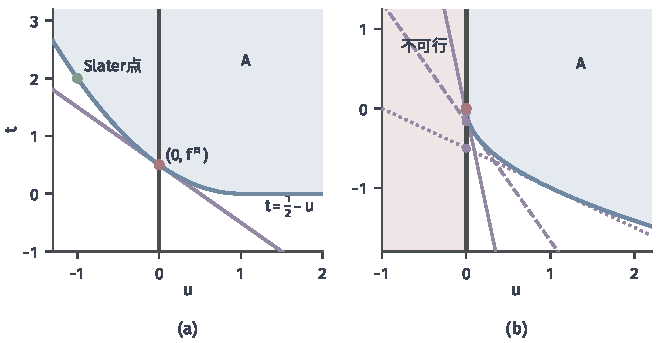
\includegraphics[width=112mm]{figures/05-optimization/06-constrained-optimization/matplotlib/dual-joint-set/figure.pdf}
 \caption{联合集合$\bm{A}$（浅蓝）与托住它的直线。(a)~一元例：紫线$t=\frac12-u$在红点$(0,f^\star)$处托住$\bm{A}$，斜率对应$\lambda^\star=1$；绿点是Slater点$x=0$对应的$(g,f)=(-1,2)$，它在竖线$u=0$的左侧。(b)~$\min x$，约束$x^2\leq u$：浅红区域$u<0$不可行，$\bm{A}$的边界在红点处切线竖直，紫线是$\lambda=0.5,1.5,5$（点线、虚线、实线）的托线，交点高度$-1/(4\lambda)$随$\lambda$增大升向$0$，但能经过红点的只有深灰色竖线。}
 \label{fig:dual-joint-set}
\end{BookInlineFigure}

要排除竖直的纸，只需要$\bm{A}$在竖线左侧确实有点，这正是图~\ref{fig:dual-joint-set}(a)中绿点起的作用。

\subsection{Slater条件}
\label{sec:dual-slater}

把上面的想法写成条件。设$f,g_i:\mathbb{R}^n\to\mathbb{R}\cup\{+\infty\}$是凸函数，等式约束仿射，写成$\bm{A}\bm{x}=\bm{b}$，其中$\bm{A}\in\mathbb{R}^{p\times n}$。共同有效定义域是
\[
 \bm{D}=\operatorname{dom}f\cap\bigcap_i\operatorname{dom}g_i.
\]
第~\ref{chap:nonsmooth-composite-optimization}章用$\operatorname{ri}$表示相对内部，即在集合自身的仿射包内的内点。

\begin{definition}[Slater条件]
 \label{def:dual-slater}
 若存在$\bar{\bm{x}}\in\operatorname{ri}\bm{D}$，使
 \begin{equation}
  g_i(\bar{\bm{x}})<0,\quad i=1,\ldots,m,\qquad\bm{A}\bar{\bm{x}}=\bm{b},
  \label{eq:dual-slater}
 \end{equation}
 就称问题满足\term{Slater条件}（Slater's condition），$\bar{\bm{x}}$称为Slater点。
\end{definition}

条件的每一部分都有用处。严格不等式让点落在竖线左侧；等式约束无法严格，只要求满足；取在相对内部，是为了让定义域在$\bar{\bm{x}}$周围留有余地，否则余量可能恰好被定义域的边缘吃掉。

三个例子都容易找到Slater点。一元例取$\bar{x}=0$，$g(\bar{x})=-1<0$。预算例取$\bar{\bm{x}}=(1/2,1/2)$，它在$\bm{D}=\mathbb{R}^2_{+}$的内部，且$x_1+x_2-2=-1<0$。二次例没有不等式，取约束直线上的任一点。

证明要分离的不是闭集，$(\bm{0},f^\star)$可能就在$\bm{A}$的边界上。定理~\ref{thm:dual-separation}不够用，需要下面这个不要求闭性、也不要求严格的版本。

\begin{lemma}[点与凸集的分离]
 \label{lem:dual-separation-convex}
 设$\bm{S}\subseteq\mathbb{R}^N$非空、凸，$\bm{z}\notin\bm{S}$。则存在$\bm{a}\neq\bm{0}$，使得对所有$\bm{w}\in\bm{S}$，
 \begin{equation}
  \langle\bm{a},\bm{w}\rangle\geq\langle\bm{a},\bm{z}\rangle.
  \label{eq:dual-separation-convex}
 \end{equation}
\end{lemma}

\begin{proof}
 $\mathbb{R}^N$的子集有可数稠密子集，取$\bm{S}$中的这样一列点$\bm{w}_1,\bm{w}_2,\ldots$。对每个$k$，令$\bm{S}_k$是$\bm{w}_1,\ldots,\bm{w}_k$的凸组合全体。

 $\bm{S}_k$是单纯形在连续映射下的像，所以是紧的，从而是闭集；它包含于凸集$\bm{S}$，所以不含$\bm{z}$。对$\bm{S}_k$用定理~\ref{thm:dual-separation}，取相反数并归一化，得到单位向量$\bm{a}_k$，使
 \[
  \langle\bm{a}_k,\bm{w}_j\rangle>\langle\bm{a}_k,\bm{z}\rangle,\qquad j=1,\ldots,k.
 \]

 单位球面是紧集，$\bm{a}_k$有收敛子列，极限$\bm{a}$仍是单位向量。固定$j$，让$k$沿子列趋于无穷，得到
 \[
  \langle\bm{a},\bm{w}_j\rangle\geq\langle\bm{a},\bm{z}\rangle.
 \]
 $\{\bm{w}_j\}$在$\bm{S}$中稠密，内积连续，所以式~\eqref{eq:dual-separation-convex}对全部$\bm{w}\in\bm{S}$成立。
\end{proof}

\begin{theorem}[Slater条件下的强对偶]
 \label{thm:dual-slater}
 设问题的$f,g_i$凸、等式约束仿射，满足Slater条件，且$f^\star$有限。则
 \begin{equation}
  d^\star=f^\star,
  \label{eq:dual-strong}
 \end{equation}
 并且对偶最优值被某组$(\bm{\lambda}^\star,\bm{\nu}^\star)$达到，其中$\bm{\lambda}^\star\geq\bm{0}$。
\end{theorem}

\begin{proof}
 第一步，选取工作空间。令$\bm{V}$是$\bm{D}$的仿射包的方向子空间，$\bm{W}=\{\bm{A}\bm{v}:\bm{v}\in\bm{V}\}$。对$\bm{x}\in\bm{D}$，由$\bm{A}\bar{\bm{x}}=\bm{b}$，有
 \[
  \bm{A}\bm{x}-\bm{b}=\bm{A}(\bm{x}-\bar{\bm{x}})\in\bm{W}.
 \]
 所以等式残差不会离开$\bm{W}$，只需要在$\mathbb{R}^m\times\bm{W}\times\mathbb{R}$中讨论。

 第二步，构造被分离的集合。令$\bm{S}$是满足下面条件的$(\bm{u},\bm{w},t)$的全体：存在$\bm{x}\in\bm{D}$，使$g_i(\bm{x})\leq u_i$，$\bm{A}\bm{x}-\bm{b}=\bm{w}$，$f(\bm{x})<t$。由$f,g_i$的凸性和等式的仿射性，$\bm{S}$是凸集，并且它是非空的，因为$\bar{\bm{x}}\in\bm{D}$。点$(\bm{0},\bm{0},f^\star)$不在$\bm{S}$中，否则存在可行点使$f(\bm{x})<f^\star$。

 第三步，应用分离。由引理~\ref{lem:dual-separation-convex}，存在不全为零的$\bm{\lambda}\in\mathbb{R}^m$、$\bm{\nu}\in\bm{W}$、$\lambda_0\in\mathbb{R}$，使对所有$(\bm{u},\bm{w},t)\in\bm{S}$，
 \[
  \langle\bm{\lambda},\bm{u}\rangle+\langle\bm{\nu},\bm{w}\rangle+\lambda_0t\geq\lambda_0f^\star.
 \]
 $\bm{S}$中的点可以把$u_i$或$t$任意增大，若$\lambda_i<0$或$\lambda_0<0$，左端会趋于$-\infty$，所以$\bm{\lambda}\geq\bm{0}$，$\lambda_0\geq0$。

 任取$\bm{x}\in\bm{D}$，取$\bm{u}=(g_i(\bm{x}))_i$，$\bm{w}=\bm{A}\bm{x}-\bm{b}$，$t=f(\bm{x})+\varepsilon$，令$\varepsilon\downarrow0$，得到
 \[
  \sum_i\lambda_ig_i(\bm{x})+\langle\bm{\nu},\bm{A}\bm{x}-\bm{b}\rangle+\lambda_0f(\bm{x})\geq\lambda_0f^\star,\qquad\bm{x}\in\bm{D}.
 \]

 第四步，证明$\lambda_0>0$，也就是这张纸不竖直。设$\lambda_0=0$。把$\bm{x}=\bar{\bm{x}}$代入上式，等式项为零，得到
 \[
  \sum_i\lambda_ig_i(\bar{\bm{x}})\geq0.
 \]
 由$g_i(\bar{\bm{x}})<0$和$\bm{\lambda}\geq\bm{0}$，只能$\bm{\lambda}=\bm{0}$。于是$\bm{\nu}\neq\bm{0}$，并且上式变成对所有$\bm{x}\in\bm{D}$，
 \[
  \langle\bm{\nu},\bm{A}(\bm{x}-\bar{\bm{x}})\rangle\geq0.
 \]
 因为$\bar{\bm{x}}\in\operatorname{ri}\bm{D}$，存在$r>0$，使对$\bm{v}\in\bm{V}$，$\lVert\bm{v}\rVert_2\leq r$，都有$\bar{\bm{x}}+\bm{v}\in\bm{D}$。代入$\pm\bm{v}$，得到$\langle\bm{\nu},\bm{A}\bm{v}\rangle=0$，也就是$\bm{\nu}$与$\bm{W}$正交。而$\bm{\nu}\in\bm{W}$，所以$\bm{\nu}=\bm{0}$，矛盾。

 第五步，构造乘子。令$\bm{\lambda}^\star=\bm{\lambda}/\lambda_0$，$\bm{\nu}^\star=\bm{\nu}/\lambda_0$，除以$\lambda_0$，上面第三步的不等式成为对所有$\bm{x}\in\bm{D}$，
 \[
  \mathcal{L}(\bm{x},\bm{\lambda}^\star,\bm{\nu}^\star)\geq f^\star.
 \]
 对$\bm{x}$取下确界，
 \[
  q(\bm{\lambda}^\star,\bm{\nu}^\star)\geq f^\star.
 \]
 由弱对偶，
 \[
  q(\bm{\lambda}^\star,\bm{\nu}^\star)\leq d^\star\leq f^\star.
 \]
 所以三者相等，并且这组乘子达到$d^\star$。
\end{proof}

证明里Slater点只在第四步用到，这正是前面“排除竖直的纸”的严格写法。定理的结论并不包括原始最优点存在，这一点在第~\ref{sec:dual-gap-attainment}节用例子说明。Slater点本身可行，所以$f^\star<+\infty$，有限的假设只是排除$f^\star=-\infty$；这时弱对偶迫使$d^\star=-\infty$，对偶可行的乘子不存在，也就谈不上最优乘子。

如果某些$g_i$本身是仿射的，这些约束不必严格满足，只要$g_i(\bar{\bm{x}})\leq0$，其余要求不变。原因在于仿射约束的集合是多面体，分离时不会出现图~\ref{fig:dual-joint-set}(b)那样切线竖直的边缘，这与线性规划不需要严格可行点的道理相同。证明需要用到多面体凸集的分离，篇幅较长，读者可查阅\scite{rockafellar1970convex}。全部约束都仿射、目标线性时，这就是第~\ref{chap:linear-programming}章已经证明的强对偶。

\subsection{共轭对偶的正则条件}
\label{sec:dual-regularity}

复合问题~\eqref{eq:dual-composite}没有不等式，不等式上的“严格可行”没有对应物，正则条件要换一种说法。回忆它的改写形式：变量$(\bm{x},\bm{z})$，有效定义域是$\operatorname{dom}f\times\operatorname{dom}g$，约束是线性等式。Slater条件要求的是存在满足等式、位于定义域相对内部的点。乘积集的仿射包是各因子仿射包的乘积，所以乘积集的相对内部等于各因子相对内部的乘积，这就翻译成了下面的条件。

\begin{theorem}[Fenchel对偶的强对偶]
 \label{thm:dual-fenchel-strong}
 设$f:\mathbb{R}^n\to\mathbb{R}\cup\{+\infty\}$，$g:\mathbb{R}^p\to\mathbb{R}\cup\{+\infty\}$是适当、下半连续的凸函数，$\bm{A}\in\mathbb{R}^{p\times n}$。若存在$\bm{x}$使
 \begin{equation}
  \bm{x}\in\operatorname{ri}(\operatorname{dom}f),\qquad\bm{A}\bm{x}\in\operatorname{ri}(\operatorname{dom}g),
  \label{eq:dual-fenchel-regular}
 \end{equation}
 且式~\eqref{eq:dual-composite}的最优值$F^\star$有限，则$\sup_{\bm{\nu}}q(\bm{\nu})=F^\star$，其中$q$由式~\eqref{eq:dual-fenchel}给出，并且对偶最优值被达到。
\end{theorem}

\begin{proof}
 把定理~\ref{thm:dual-slater}用于改写形式，变量是$(\bm{x},\bm{z})$，目标是$f(\bm{x})+g(\bm{z})$，等式是$\bm{A}\bm{x}-\bm{z}=\bm{0}$，没有不等式。若$\bm{x}$满足式~\eqref{eq:dual-fenchel-regular}，则$(\bm{x},\bm{A}\bm{x})$在定义域的相对内部且满足等式，是Slater点。改写形式的对偶函数正是式~\eqref{eq:dual-fenchel}。
\end{proof}

证明中没有用到下半连续。这个假设保证$f^{**}=f$和$g^{**}=g$，使$q$对应的对偶问题再取一次对偶时能回到原问题，所以通常写在一起。定理保证的是两个最优值相等、对偶最优乘子存在，原始问题的最小点是否存在，要另外用强制性或紧性论证。

上一节的绝对值例中$\operatorname{dom}f=\mathbb{R}^2$，$\operatorname{dom}g=\mathbb{R}$，两个定义域都是全空间，条件自动满足，所以那里的零间隙在算出结果之前就可以预知。

条件中的相对内部不是形式要求，看一个定义域只在边界上相遇的例子。取$f(x)=-\sqrt{x}$（$x\geq0$，其余为$+\infty$），$g=\iota_{\{0\}}$，$A=1$。此时要求$x\in(0,\infty)$且$x=0$，式~\eqref{eq:dual-fenchel-regular}不成立。可行点只有$x=0$，所以$F^\star=0$。

对偶一侧，$g^*=0$。$\nu>0$时$f^*(-\nu)=\sup_{x\geq0}\{-\nu x+\sqrt{x}\}$在$\sqrt{x}=1/(2\nu)$处达到，于是
\[
 f^*(-\nu)=\frac{1}{4\nu},\qquad q(\nu)=-\frac{1}{4\nu}.
\]
$\nu\leq0$时$f^*(-\nu)=+\infty$。所以$\sup q=0=F^\star$，零间隙仍然成立，但上确界取不到，对偶最优乘子不存在。

\subsection{间隙与达到的区别}
\label{sec:dual-gap-attainment}

“强对偶成立”“原始最优点存在”“最优乘子存在”是三件不同的事。本小节用三个例子分别让其中一件出问题，表~\ref{tab:dual-gap-cases}是它们的汇总。

第一个例子最小化$e^{-x}$，约束$-x\leq0$。Slater点$x=1$存在，$f^\star=0$有限，定理~\ref{thm:dual-slater}适用。第~\ref{sec:dual-function}节已经算出$q(0)=0$，其余$q(\lambda)=-\infty$，于是
\[
 d^\star=0=f^\star,\qquad\lambda^\star=0.
\]
零间隙成立，乘子达到，但没有$x$能使$e^{-x}=0$，原始最优值不达到。图~\ref{fig:dual-three-failures}(a)是这个函数，它只在无穷远处靠近下确界。

第二个例子最小化$x$，约束$x^2\leq0$。唯一的可行点是$x=0$，所以$f^\star=0$，原始最优点存在。Slater条件不成立，因为$x^2<0$无解。

对$\lambda>0$，$x+\lambda x^2$在$x=-1/(2\lambda)$处最小，$\lambda=0$时下确界为$-\infty$。于是
\[
 q(\lambda)=-\frac{1}{4\lambda}\quad(\lambda>0).
\]
$\lambda\to+\infty$时$q\to0$，所以$d^\star=0=f^\star$，零间隙成立，但没有有限的$\lambda$能达到。如图~\ref{fig:dual-three-failures}(b)，这正是图~\ref{fig:dual-joint-set}(b)中切线竖直的代价。

这个例子还说明，第~\ref{chap:constrained-optimality}章在同一问题上看到的“最小点没有KKT乘子”，与“对偶最优值取不到”是同一件事的两面。

第三个例子的定义域是$\bm{D}=\{\bm{x}\in\mathbb{R}^2:x_2>0\}$，问题是
\[
 \min_{\bm{x}\in\bm{D}}\ e^{-x_1}\quad\text{s.t.}\quad\frac{x_1^2}{x_2}\leq0.
\]
函数$x_1^2/x_2$在$x_2>0$上是凸的，这可以由Hessian半正定验证，所以这是一个凸问题。约束迫使$x_1=0$，于是$f^\star=1$，并在$\{0\}\times(0,\infty)$上达到。

求对偶函数。对任意$\lambda\geq0$，内层函数$e^{-x_1}+\lambda x_1^2/x_2$总是正的，所以$q(\lambda)\geq0$。沿曲线$x_1=s$，$x_2=s^3$，令$s\to+\infty$，有
\[
 e^{-s}+\frac{\lambda}{s}\to0.
\]
所以$q(\lambda)=0$对所有$\lambda\geq0$成立，$d^\star=0$。

两个最优值分别是$1$和$0$，对偶间隙为$1$。这说明凸性本身不能保证零间隙。Slater条件在这里失败，因为$x_1^2/x_2<0$无解。

图~\ref{fig:dual-three-failures}(c)显示了联合集合的样子：最优值函数$v$在$u=0$处的值是$1$，而$u>0$时只要让$x_1,x_2$都增大，就有$x_1^2/x_2\leq u$，目标值可以任意接近$0$，所以$v(u)=0$。$v$在$u=0$处有一个跳跃，从下方托住$\bm{A}$的直线最高只能到$0$。

\begin{BookInlineFigure}
 \centering
 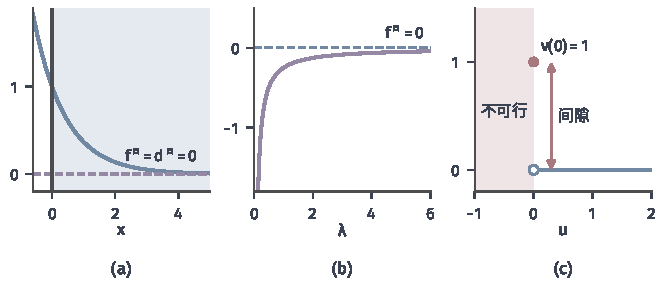
\includegraphics[width=112mm]{figures/05-optimization/06-constrained-optimization/matplotlib/dual-three-failures/figure.pdf}
 \caption{三种不同的情形。(a)~蓝线是$e^{-x}$，浅蓝区域可行，下确界$0$不被取到，紫色虚线是$d^\star$。(b)~$\min x$，约束$x^2\leq0$的对偶函数$q(\lambda)=-1/(4\lambda)$，向蓝色虚线$f^\star=0$靠近但取不到。(c)~第三个例子的最优值函数：浅红区域$u<0$不可行，红点是$v(0)=1$，$u>0$时$v(u)=0$，空心点表示$u=0$时下极限，红色箭头是对偶间隙$1$。}
 \label{fig:dual-three-failures}
\end{BookInlineFigure}

\begin{BookInlineTable}
 \centering
 \begin{tabular}{@{}llllll@{}}
  \toprule
  问题 & Slater & $f^\star$ & $d^\star$ & 原始达到 & 对偶达到\\
  \midrule
  $\min e^{-x}$，$-x\leq0$ & 成立 & $0$ & $0$ & 否 & 是\\
  $\min x$，$x^2\leq0$ & 不成立 & $0$ & $0$ & 是 & 否\\
  $\min e^{-x_1}$，$x_1^2/x_2\leq0$ & 不成立 & $1$ & $0$ & 是 & 是\\
  \bottomrule
 \end{tabular}
 \caption{间隙与达到的三个例子。第三个例子全部乘子都是对偶最优的。}
 \label{tab:dual-gap-cases}
\end{BookInlineTable}

表中第二行和第三行都不满足Slater条件，结局却不同：一个零间隙，一个正间隙。所以Slater条件只是充分条件，不成立时要具体分析。
